\documentclass[a4paper,14pt]{extreport}
	\usepackage[left=1.5cm,right=1.5cm,
	    top=1.5cm,bottom=2cm,bindingoffset=0cm]{geometry}
	\usepackage{scrextend}
	\usepackage[T1,T2A]{fontenc}
	\usepackage[utf8]{inputenc}
	\usepackage[english,russian,ukrainian]{babel}
	\usepackage{tabularx}
	\linespread{1.5}
	\usepackage{amssymb}
	\usepackage{fp}
	\usepackage{color}
	\usepackage{amsmath}
	\usepackage{mathrsfs}
	\usepackage{listings}
	\usepackage{graphicx}
	\graphicspath{ {./images/} }
	\usepackage{lipsum}
	\usepackage{xcolor}
	\usepackage{multirow}
	%\usepackage[table,xcdraw]{xcolor}
	\usepackage{hyperref}
	\usepackage{tcolorbox}
	\usepackage{tikz}
	\usepackage[framemethod=TikZ]{mdframed}
	\usepackage{wrapfig,boxedminipage,lipsum}


\begin{document}
\newtcbox{\xmybox}[1][red]{on line, arc=7pt,colback=#1!10!white,colframe=#1!50!black, before upper={\rule[-3pt]{0pt}{10pt}},boxrule=1pt, boxsep=0pt,left=6pt,right=6pt,top=2pt,bottom=2pt}

\begin{titlepage}
	\begin{center}
	\large
	Національний технічний університет України \\ "Київський політехнічний інститут імені Ігоря Сікорського"


	Факультет Електроніки

	Кафедра мікроелектроніки
	\vfill

	\textsc{ЗВІТ}\\

	{\Large Про виконання лабораторної роботи №3\\
	з дисципліни: «Функціональна електроніка»\\[1cm]

	Дослiдження оптоелектронного перетворювача
зображення

	}
	\bigskip
	\end{center}
	\vfill

	\newlength{\ML}
	\settowidth{\ML}{«\underline{\hspace{0.4cm}}» \underline{\hspace{2cm}}}
	\hfill
	\begin{minipage}{1\textwidth}
	Виконавець:\\
	Студент 4-го курсу \hspace{4cm} $\underset{\text{(підпис)}}{\underline{\hspace{0.2\textwidth}}}$  \hspace{1cm}А.\,С.~Мнацаканов\\


	Перевірив: \hspace{5.9cm} $\underset{\text{(підпис)}}{\underline{\hspace{0.2\textwidth}}}$  \hspace{1cm}С.\,В.~Малюта\\

	\end{minipage}

	\vfill

	\begin{center}
	2021
	\end{center}
\end{titlepage}






\textbf{Мета роботи} - Дослiдження передавальних характеристик оптоелектронного перетворюва-
ча зображення.

\begin{center}
Завдання 
\end{center}

1. Зiбрати схему стенда для вимiрювання параметрiв оптронного перетворювача
зображення.\\
2. Ввiмкнути джерело напруги вхiдного ланцюга дослiджуваної схеми та джерело
напруги змiщення вихiдного ланцюга.\\
3. Виставити на джерелi напруги вихiдного ланцюга схеми
 Uзм1
 (значення задається викладачем).\\
4. Пiдключити позитивну клему вихiдного вимiрювального ланцюга до гнiзда 4.\\ 
5. Змiнюючи вхiдний струм (дiапазон та крок задається викладачем) вимiряти
струм у вихiдному ланцюгу для червоного свiтлодiода. Вiдмiтити струм загоряння
свiтлодiода.\\ 
6. Пiдключити позитивну клему вихiдного вимiрювального ланцюга до гнiзда 5.
Повторити п.5 для зеленого свiтлодiода.\\ 
7. Пiдключити позитивну клему вихiдного вимiрювального ланцюга до гнiзда 6.
Повторити п.5 для жовтого свiтлодiода.\\ 
8. Виставити на джерелi напруги вихiдного ланцюга схеми
 Uзм2
 (значення задається викладачем). Повторити п. 5-7.\\ 
9. Виставити на джерелi напруги вихiдного ланцюга схеми
 Uзм3
 (значення задається викладачем). Повторити п. 5-7.\\ 
10. Вимкнути джерела напруги.\\ 
\begin{figure}[h]
	\center{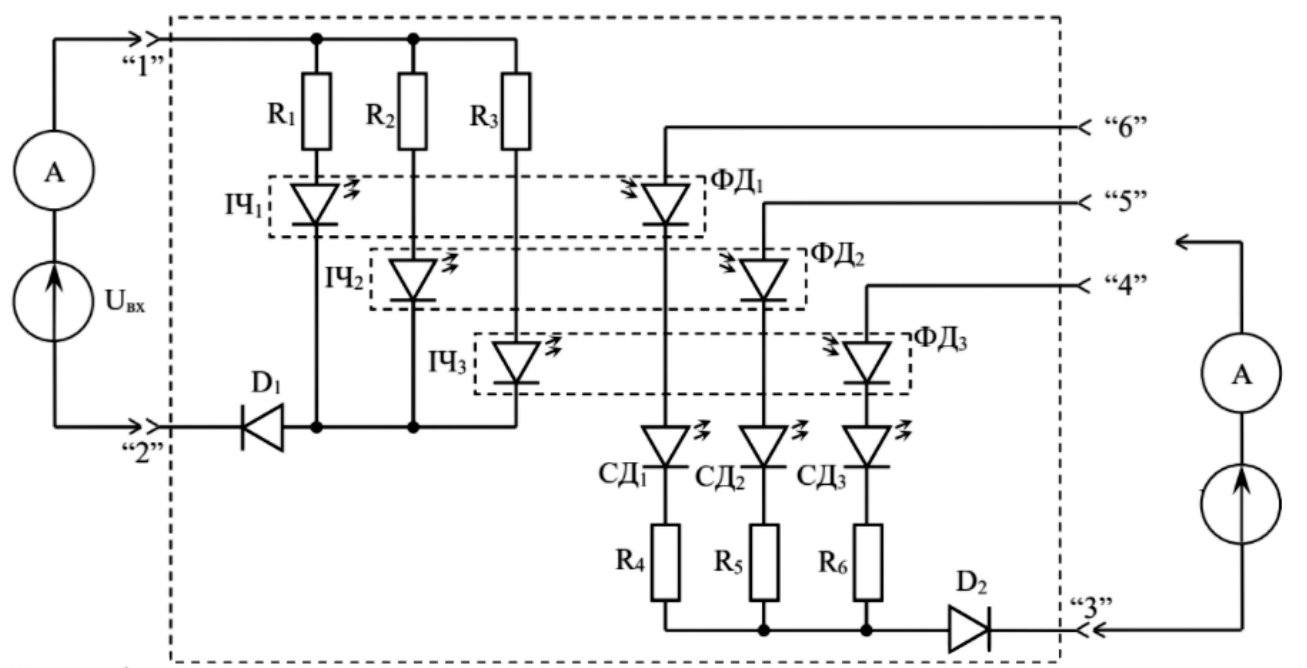
\includegraphics[width=0.7\linewidth]{1.png}}
	\caption{ Схема для дослiдження передавальних х-к оптоелектронного перетворювача.}
	\label{ris1}
\end{figure}





\begin{figure}[h]
\begin{center}
Результати вимiрювань 
\end{center}
\caption{ Табл. 1: Результат вимiрювання струму у вихiдних ланцюгах свiтлодiодiв.}
	\center{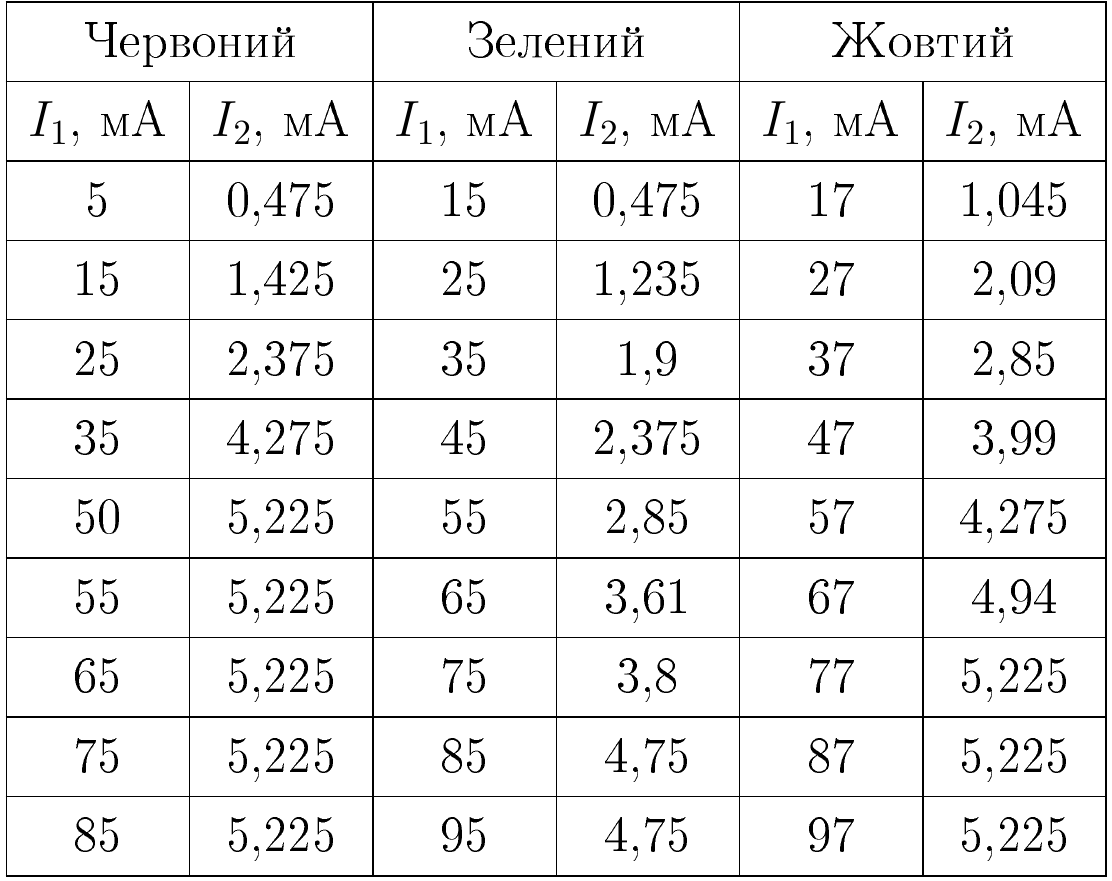
\includegraphics[width=0.6\linewidth]{2.png}}
	\label{ris2}
\end{figure}

\begin{figure}[h]
\begin{center}
Графік
\end{center}
	\center{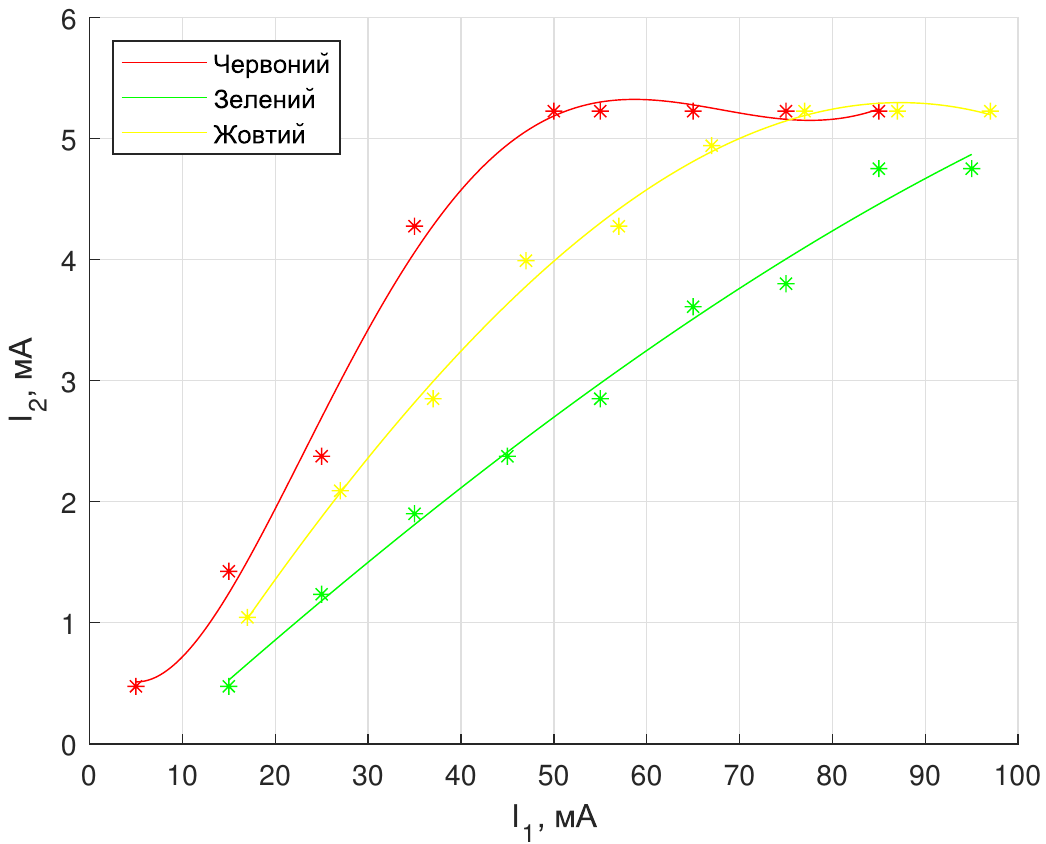
\includegraphics[width=0.7\linewidth]{3.png}}
	\caption{ Залежнiсть струму у вихiдному ланцюгу вiд струму через iнфрачервонi свiтлодiоди.}
	\label{ris1}
\end{figure}

\clearpage
\begin{center}
Висновок
\end{center}

Аналiзуючи результати вимiрювань маємо наступне:\\ 

-- найменший струм загоряння має червоний свiтлодiод (5 мА), найбiльший -
жовтий (17 мА).\\

-- передавальна характеристика для усiх свiтлодiодiв є бiльш-менш лiнiйною.\\ 

-- при подальшому збiльшеннi вхiдного струму струм у вихiдному ланцюзi для
свiтлодiюдiв практично не змiнюється.\\ 

-- червоний свiтлодiод має найкрутiший характер передавальної характери-
стики, а зелений - найменший, отже найбiльший коефiцiєнт передачi має
червоний свiтлодiод, найменший - зелений.
\begin{figure}[h!]
	\center{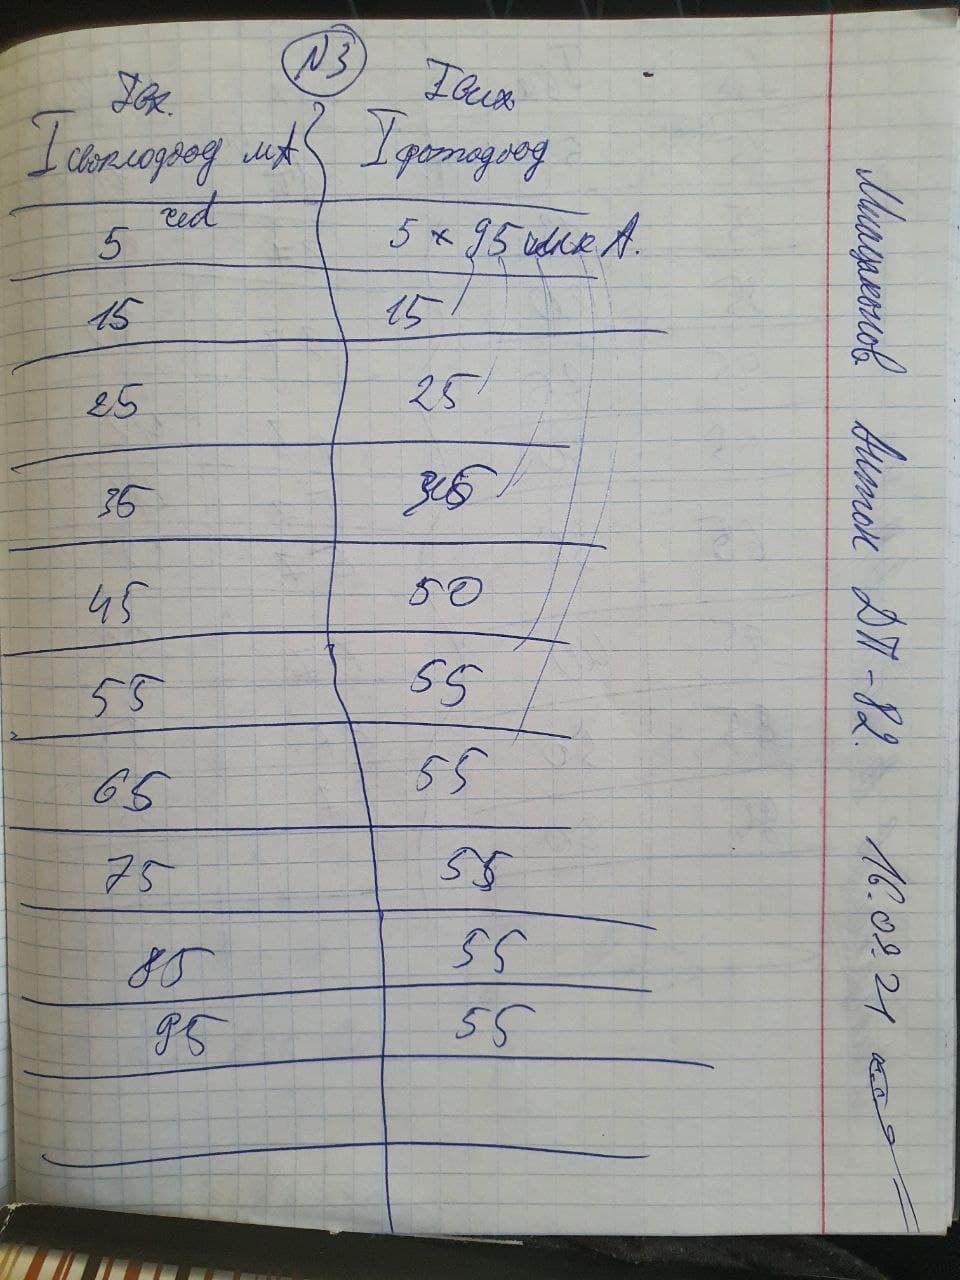
\includegraphics[width=0.7\linewidth]{22.jpg}}
\end{figure}

\end{document}

